\documentclass[]{cv-etienne}

\usepackage[italian, american]{babel}

\usepackage[autostyle]{csquotes}
%\usepackage{graphix}

\usepackage{fontawesome}

\addbibresource{curriculum.bib}


\hypersetup{%
  colorlinks=false,% hyperlinks will be black
  linkbordercolor=red,% hyperlink borders will be red
  pdfborderstyle={/S/U/W 1}% border style will be underline of width 1pt
}

\newfontfamily{\FA}{FontAwesome Regular}


\begin{document}
\header{Etienne}{Delay}{Chercheur en géographie sociale et modélisation spatiale}

\begin{aside} % In the aside, each new line forces a line break
%\includegraphics[width=largeur]{nom du fichier}
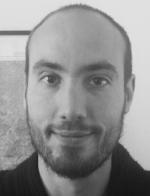
\includegraphics{img/delay_s}
\section{Personnel}
Âge : 32 ans
Situation : Pacsé
\section{Contact}
Villa 127
Sacré c\oe{}ur 3 Pyrotechnie
Dakar, Sénégal.
~
+33 614 325 300
+221 77 459 90 43
~
{\color{lightgray}{\FA \faEnvelope}} \href{mailto:etienne.delay@gmail.com}{\footnotesize etienne.delay@gmail.com}
{\color{linkedin}{\FA \faLinkedin}} \href{https://fr.linkedin.com/in/etienne-delay-8871a45b}{\footnotesize http://goo.gl/InWAhm}
{\color{twitter}{\FA \faTwitter}} {\footnotesize \href{https://twitter.com/ElCep}{@ElCep}}
{\color{github}{\FA \faGithub}} {\footnotesize \href{https://github.com/ElCep}{ElCep}}
{\color{lightgray}{\FA \faHome}} {\footnotesize \href{http://elcep.legtux.org}{http://lamenagerie.org}}
\section{Langages}
Français : langue\\ maternelle
Anglais : scolaire
Italien : avancé
\section{Programmation}
{\color{red} $\varheartsuit$} R, Netlogo
SQL et dialectes
\LaTeX, markdown,
formalisme UML.
\section{Logiciels}
{\color{red} $\varheartsuit$} Linux \& Unix-like,
Netlogo, {\color{red} $\varheartsuit$} OpenMOLE,
{\color{red} $\varheartsuit$} Gama-platefrome,
GIT,QGIS, GRASS, Mapserver, GeoServer,
PostgreSQL, PostGIS,
pgRouting, MySQL
\end{aside}

\section{Intérêts}
Pour faire face aux défis scientifiques proposés par les dynamiques des paysages et les processus de coopération, j'ai développé une méthodologie de recherche basée sur le travail de terrain et la modélisation co-construite, combinée à la formalisation des processus et des modèles à base d'agents.
Cette approche offre la possibilité de comprendre les conditions spatiales, sociales, culturelles et économiques qui s'inscrivent sur les territoires afin de proposer des scénarios prospectifs.
Ces méthodes ont été appliquées dans des contextes variés: sur les paysages de vignobles de fortes pentes (2011), sur la coopération pour la gestion des ressources en eau (2015), sur la couverture végétale en climat sahélien (2017).
Les réseaux de recherche fortement interdisciplinaires que j'ai pu établir dans ces différents contextes sont toujours actifs grâce à des collaborations et des activités soutenues.

Mon expertise technique, thésaurisée tout au long de mon cursus universitaire, s'est ensuite développée grâce à mon investissement dans plusieurs groupes de travail: au sein de l'équipe MAPS (Modélisation appliquée aux phénomènes spatiaux), du projet OpenMOLE, de l'association OSGeo (président du chapitre français OSGeo depuis 2013, membre du chapitre OSGeo-international depuis 2015), et lors de diverses initiatives autour de la modélisation à base d'agents, de l'exploration et de l'analyse de la sensibilité des comportements des modèles spatiaux. Plus généralement je m'investis fortement dans les communautés des logiciels libres.

J'aime les voyages, la zététique, la science-fiction dystopique et la course à pied.

\section{Projets}
\begin{entrylist}
%------------------------------------------------
\entry
{Depuis 2017}
{ANR Future Sahel {\normalfont dirigée par D. Goffner}}
{UMI 3189 CNRS, Dakar, SNG}
{Le programme \emph{Future Sahel} est financé par l'ANR. Son objectif est de fournir une aide scientifique et technique à l'agence nationale de la grande muraille verte au Sénégal.}
%------------------------------------------------
\end{entrylist}
\begin{entrylist}
%------------------------------------------------
\entry
{2016}
{Programme COMMONS {\normalfont dirigé par M. Chevallier et E. Delay}}
{UMR 6042 CNRS, Laboratoire Geolab, FR}
{\emph{Le programme COMMONS "\textit{COllective ManageMent Of Natural reSources}"} est financé par l'AOI de l'université de Limoges et la fondation partenariale de l'université. Objectif : structurer un réseau de partenaires internationaux pour engager une approche interdisciplinaire autour des processus de gestion collective des ressources naturelles.}
%------------------------------------------------
\end{entrylist}
\begin{entrylist}
%------------------------------------------------
\entry
{Depuis 2015}
{Projet LittoSim {\normalfont dirigé par N. Becu}}
{UMR 7266 CNRS, Laboratoire LIENs, FR}
{\emph{Le projet LittoSim} a été financé dans le cadre du "Défi Littoral 2015" du CNRS et a rassemblé 11 chercheurs français. Objectif : développement d'un outil pédagogique permettant de sensibiliser les aménageurs du territoire aux mesures de prévention et d'aménagement liées au risque de submersion marine.}
%------------------------------------------------
\end{entrylist}
\begin{entrylist}
%------------------------------------------------
\entry
{2014-2016}
{Programme VitiTerroir {\normalfont dirigé par S. Leturcq et A. Lammoglia}}
{LAT-UMR 7324 CITERES, FR}
{\emph{Le programme VitiTerroir} propose d'initier un outil prospectif fondé sur une modélisation des transformations des terroirs viticoles dans la longue durée.}
%------------------------------------------------
\end{entrylist}
\begin{entrylist}
%------------------------------------------------
\entry
{2012 -- 2015}
{Programme LACCAVE {\normalfont dirigé par N. Ollat et J-M. Touzard}}
{INRA, FR}
{Le programme \emph{Long term impacts and Adaptation to Climate ChAnge in Viticulture and Enology} rassemble 23 laboratoires de recherche en France, pour évaluer les effets du changement climatique sur la vigne et explorer les stratégies d'adaptation mobilisables.}
%------------------------------------------------
\end{entrylist}
\begin{entrylist}
%------------------------------------------------
\entry
{Depuis 2011}
{Ricerca sulla viticoltura di montagna  {\normalfont  dirigé par M. Pontalti et F. Zottele \\}}
{ Fondazione E.MACH, IT}
{\emph{Études et expérimentation pour le maintien d'une viticulture de montagne dans le Trentino et plus largement sur des problématiques européennes}, en partenariat avec le CERVIM  (Centre d'études et de recherche sur la viticulture de montagne).}
%------------------------------------------------
\end{entrylist}
\begin{entrylist}
%------------------------------------------------
\entry
{2011 -- 2015}
{ANR TerViClim {\normalfont dirigé par H. Quénol}}
{ Université de Rennes, FR}
{\emph{Observation et spatialisation du climat des terroirs viticoles mondiaux dans un contexte de changement climatique} :
Installation de capteurs de température sur l'AOC Banyuls-Collioure (Pyrénées Orientales, FR) et dans le Val Di Cembra (Trentino, IT).}
%------------------------------------------------
\end{entrylist}
%\pagebreak
\section{Responsabilités scientifiques}
\begin{entrylist}
%------------------------------------------------
\entry
{Juin 2017}
{Co-organisateur de l'école thématique CNRS MAPS10}
{CAES CNRS - Olérons}
{Ecole thématique labellisée par le CNRS. Pour 30 participants, une semaine de formation qui consiste à former au développement de modèles spatialisés de phénomènes sociaux-environnementaux.}
%------------------------------------------------
\end{entrylist}
\begin{entrylist}
%------------------------------------------------
\entry
{Juin 2017}
{Membre du comité scientifique pour le $20^{e}$ congrès international du GiESO}
{UNCUYO - Mendoza (ARG)}
{Ce congrès est un lieu d'échange sur les principaux domaines des sciences et technologies de la viticulture.}
%------------------------------------------------
\end{entrylist}
\begin{entrylist}
%------------------------------------------------
\entry
{Oct. 2016}
{Membre du comité scientifique de l'atelier : "formes alternatives de participation à la démocratie de l'eau"}
{FLSH - Limoges}
{Atelier de 3 jours en vue de produire un état de l'art des formes de gouvernance participative dans la démocratie de l'eau et d'identifier les formes de participation alternatives. Cet atelier réunit 20 chercheurs internationaux.}
%------------------------------------------------
\end{entrylist}
\begin{entrylist}
%------------------------------------------------
\entry
{Depuis 2015}
{Membre du noyau MAPS}
{}
{MAPS est un réseau thématique de modélisations multi-agents appliquées aux phénomènes spatialisés qui regroupe une centaine de chercheurs. Le noyau est constitué de 12 chercheurs s'investissant dans l'organisation et l'animation du réseau. Tous les ans, nous organisons des ateliers de modélisation interdisciplinaires ayant pour objectif de développer des simulations dans le champ des systèmes complexes spatialement explicites.}
%------------------------------------------------
\end{entrylist}
\begin{entrylist}
%------------------------------------------------
\entry
{Depuis 2015}
{Membre de l'équipe OpenMOLE}
{ISC-PIF - Paris}
{OpenMOLE est une plateforme qui vise à fournir à ses utilisateurs un ensemble d'outils d'exploration, de diagnostic et d'optimisation de modèles numériques.}
%------------------------------------------------
\end{entrylist}
\begin{entrylist}
%------------------------------------------------
\entry
{Juin 2015}
{Membre du comité scientifique pour le $19^{e}$ congrès international du GiESCO}
{Palais des congrès - Gruissan}
{Ce congrès est un lieu d'échanges sur les principaux domaines des sciences et technologies de la viticulture. Cet événement a rassemblé 250 scientifiques et ingénieurs de 20 pays, afin de mettre en lumière les dernières avancées en viticulture pour en faciliter le transfert vers les autres disciplines et le monde professionnel.}
%------------------------------------------------
\end{entrylist}
\begin{entrylist}
%------------------------------------------------
\entry
{Depuis 2014}
{Coordinateur du FOSS4G-eu}
{ENSG - Marne-la-Vallée}
{\emph{Free and Open Source Software for Geospatial congress} (FOSS4G). Cette conférence de 3 jours, réunit les communautés européennes des utilisateurs et des développeurs intéressées par les données spatiales, les logiciels, et les applications ouvertes autour de la géomatique. Elle a eu lieu en mai 2014 et 2016 ainsi qu'en juin 2017 pour une version Européenne.}
%------------------------------------------------
\end{entrylist}
\begin{entrylist}
%------------------------------------------------
\entry
{Nov. 2013}
{Co-organisateur de l'atelier LACCAVE "agent based modeling and  multi-model coupling"}
{SupAgro - Montpellier}
{Le but de cet atelier pluridisciplinaire était de produire des modèles disciplinaires pour travailler plus spécifiquement sur le couplage de modèles.}
%------------------------------------------------
\end{entrylist}
\begin{entrylist}
%------------------------------------------------
\entry
{Juin 2013}
{Organisateur du séminaire LACCAVE}
{mas Reig - Banyuls}
{Dans le contexte du projet LACCAVE, j'ai organisé un séminaire sur l'adaptation au changement climatique en viticulture. Il s'agissait de proposer un lieu d'échange entre chercheurs et professionnels de la filière viticole autour des avancées proposées par la communauté scientifique.}
%------------------------------------------------
\end{entrylist}
\begin{entrylist}
%------------------------------------------------
\entry
{Juin 2013}
{Coordinateur du comité scientifique pour le FROG  (\emph{FRench OpenSource for Geographer})}
{IGN - Saint-Mandé}
{Une journée de conférence autour des pratiques de géomatique libre pour rassembler la communauté des utilisateurs et des développeurs.}
%------------------------------------------------
\end{entrylist}
%\vspace{15ex}

\section{Cursus universitaire}
\begin{entrylist}
%------------------------------------------------
\entry
{2011-2015}
{Doctorat de géographie {\normalfont GEOLAB UMR 6042 CNRS}}
{ Université de Limoges, FR}
{\emph{\'Evolution et prospectives paysagères des territoires viticoles de forte pente} \\Dans cette thèse, j'ai travaillé sur les possibilités prospectives, spatiales et temporelles offertes par la co-construction de modèles à base d'agents avec les acteurs locaux. Thèse réalisée sous la direction d'\'Eric \textsc{Rouvellac}, Nicolas \textsc{Becu} et Philippe \textsc{Allée}. Thèse qualifiée au CNU (section 23) en janvier 2016.}
%------------------------------------------------
\end{entrylist}

\begin{entrylist}
%------------------------------------------------
\entry
{2009-2011}
{DEUST {\normalfont "Webmaster et gestionnaire d’intranet"}}
{Université de Limoges, FR}
{\emph{Apprentissage des outils, des langages du web et de la gestion de réseaux.}}
%------------------------------------------------
\end{entrylist}

\begin{entrylist}
%------------------------------------------------
\entry
{2008-2011}
{L3, M1, M2 {\normalfont "Valorisation du patrimoine et aménagement territorial"}}
{ Université de Limoges, FR}
{\emph{Développement territorial des espaces ruraux.}}
%------------------------------------------------
\end{entrylist}

\begin{entrylist}
%------------------------------------------------
\entry
{2006-2008}
{BTSA {\normalfont Gestion et Protection de la Nature }}
{ CFPPA, la Côte-Saint-André, FR}
{\emph{Spécialité Gestion des espaces naturels (en apprentissage).}}
%------------------------------------------------
\end{entrylist}

\begin{entrylist}
%------------------------------------------------
\entry
{2004-2006}
{L1 \& L2 de Biologie}
{ Université Joseph Fourier, Grenoble, FR}
{\emph{Spécialité : modélisation des phénomènes naturels (R-project \& Berkley Madonna).}}
%------------------------------------------------
\end{entrylist}

\section{Expériences professionnelles}
\begin{entrylist}
%------------------------------------------------
\entry
{Depuis 2017}
{Post-doctorat, OHMi Téssékéré  {\normalfont sous la direction de J.-L. Peiry} ~}
{CNRS - Dakar, SNG}
{Développement d'outils d'aide à la décision et à la médiation pour les acteurs impliqués dans le projet de la Grande Muraille Verte. Ce poste s'intègre à l'ANR futur-Sahel et est basé à Dakar. Contrat de 12 mois.}
%------------------------------------------------
\end{entrylist}
\begin{entrylist}
%------------------------------------------------
\entry
{Mars 2016}
{Centre doctorales IBN ZOHR}
{Université IBN ZOHR Agadir, MA}
{\emph{Chargé de cours} \\
Co-animation d'une semaine de formation à la modélisation multi-agents à destination des doctorants de l'école doctorale IBN ZOHR à Agadir.
}
\end{entrylist}
\begin{entrylist}
%------------------------------------------------
\entry
{2015-2017}
{Post-doctorat, Chaire d'excellence "Capital environnemental et gestion durable des cours d'eau"  {\normalfont dirigé par J. Linton} ~}
{Fondation de l'université de Limoges \& Laboratoire GEOLAB UMR 6042 CNRS}
{Projet de recherche autour de l'émergence de la coopération basée sur les collectifs d'irrigants dans le département des Pyrénées-Orientales. Contrat de 16 mois.}
%------------------------------------------------
\end{entrylist}
\begin{entrylist}
%------------------------------------------------
\entry
{2015}
{Pôle d'appui à la recherche}
{Université de Limoges, FR}
{\emph{Ingénieur d'étude} \\
Mise en place de l'infrastructure informatique pour proposer de la cartographie dynamique pour l'université, basée sur Debian, Mapserver, MySQL, Openlayer3 et Leaflet. Contrat de 6 mois.
}
\end{entrylist}

\begin{entrylist}
%------------------------------------------------
\entry
{2013--2016}
{Département de géographie}
{Université de Limoges, FR}
{\emph{Chargé de cours} \\
Chargé de 80 heures de TD en statistique (avec R) pour les L1 de Géographie (40h), et en géomatique (avec Qgis, GRASS-GIS, R) pour les M2 de Géographie/Histoire/Sociologie (20h). J'ai également assuré deux modules (10h chacun) à destination des M2 SHS et portant respectivement sur l’acquisition d’outils et méthodes de recherche innovante en sciences sociales : jeux sérieux et analyse de réseaux sociaux. A chaque fois, les cours s'effectuent en présentiel et s'accompagnement d'un support électronique sur la plateforme de e-learning (moodle 2.X) de l'université.
}
\end{entrylist}
%------------------------------------------------
\begin{entrylist}
\entry
{2011}
{Fondazion E. Mach}
{San Michele all Adige, IT}
{\emph{Ingénieur d'étude}\\
Gestion de projet complet, de l'étude d'avant-projet à la mise en place du prototype d'infrastructure de serveurs cartographiques. Travail sur des données LIDAR pour la détection de formes viticoles à l'échelle du Trentino (Italie). Contrat de 8 mois.
}
\end{entrylist}
%------------------------------------------------
\begin{entrylist}
\entry
{2010}
{CERVIM}
{Aoste, IT}
{\emph{Stage}\\
Stage de 6 mois au CERVIM. Mise en place de méthodes d'inventaire par télédétection basées sur des logiciels Open Source (Qgis, GRASS, R), mise en place d’une plateforme de travail collaborative (Drupal et OpenAtrium).
}
\end{entrylist}
%------------------------------------------------
\begin{entrylist}
\entry
{2009}
{Centre d'Ampélographie Alpine}
{Cevin, FR}
{\emph{Stage}\\
Stage de 3 mois au CAAPG (Centre d'Ampélographie Alpine Pierre Galet). Mise en place de méthodes d'inventaire, mise en place du SIG, gestion du centre de documentation.
}
\end{entrylist}
%------------------------------------------------
\begin{entrylist}
\entry
{2006-2008}
{La Trace}
{Espace Naturel Sensible des Ecouges, FR}
{\emph{Apprentissage}\\
Expérimentations de gestion des espaces ouverts de l'ENS des Ecouges (Vercors).
}
\end{entrylist}
%------------------------------------------------
%\pagebreak
\section{Publications}
%\printbibsection{article}{Articles dans des revues à comité de lecture}
\begin{refsection}
  \nocite{*}
  \printbibliography[type=article,title={Articles dans des revues à comité de lecture},heading=subbibliography,sorting=ynt]
  \nocite{*}
  \printbibliography[type=incollection,title={Chapitres de livre},heading=subbibliography,sorting=ynt]
  \nocite{*}
  \printbibliography[type=inproceedings,title={Conférences/posters},heading=subbibliography,sorting=ynt]
\end{refsection}
%------------------------------------------------
\section{Dev. informatique}
Je présente ici une sélection de quelques programmes informatiques réalisés depuis le début de ma thèse. Ils mobilisent différents langages et formalismes. La plupart des développements auxquels j'ai participé sont accessibles sur mon compte github.

%------------------------------------------------
\begin{entrylist}
\entry
{2012-2015}
{Modèles de thèse}
{NetLogo, R, Slurm, openMOLE}
{
Six modèles à base d'agents co-construits avec les acteurs et développés avec NetLogo. Quatre modèles parmi ces 6 ont été publiés dans des journaux à comité de lecture (Cybergeo, Journal of Alpine Research, Land Use Policy). Ces six modèles ont servi de base à une analyse prospective des territoires de fortes pentes.  Source : \url{https://github.com/ElCep/these_ed/}.
}
\end{entrylist}
%------------------------------------------------
\begin{entrylist}
\entry
{2014}
{Température et dataVIz}
{R, shiny, postgreSQL}
{
Une application web basée sur R et \textit{shiny} pour permettre aux viticulteurs de suivre l'historique des données climatiques enregistrées sur leurs parcelles. Source : \url{https://elcep.shinyapps.io/shiny_static/}.
}
\end{entrylist}
%------------------------------------------------
\begin{entrylist}
\entry
{2014}
{QRClassInt}
{R,Qgis}
{
Un plug-in Qgis qui permet de calculer différentes formes de discrétisation pour faire des classifications cartographiques qui aient du sens.  Source : \url{https://github.com/ElCep/QRclassInt}.
}
\end{entrylist}
%------------------------------------------------
\begin{entrylist}
\entry
{2015}
{Serveur carto}
{MapServer, Openlayer3, leaflet}
{
Développement d'une architecture client-serveur pour des données géographiques pour le pôle d'appui à la recherche. L'objectif étant de permettre l'intégration de données issues de sources hétérogènes (PostgreSQL, MySQL, raster) dans un outil de visualisation adapté au web via les protocoles WMS, WFS, WPS (MapServer, OpenLayer).Source: \url{https://github.com/ElCep/htmlMap}.
}
\end{entrylist}
%------------------------------------------------
\begin{entrylist}
\entry
{2016}
{WAT-a-GAME GUI}
{R, Shiny}
{
Le jeu WAG est développé au sein de l'UMR G-EAU depuis quelques années. Pour les besoins de la chaire "capital environnemental et gestion durable des cours d'eau", j'ai développé une application web basée sur R qui permet de facilement et rapidement débriefer les ateliers. Source: \url{https://github.com/ElCep/WAT-a-Game}
}
\end{entrylist}
%------------------------------------------------
\begin{entrylist}
\entry
{depuis 2016}
{LittoSim}
{Gama, R, Shiny}
{
Jeux sérieux développés dans le cadre de l'appel à projets Défis Littoral du CNRS en 2016 et depuis 2017 par la fondation de France. Nous avons développé une architecture de jeux distribuée entre un serveur et des modèles satellites sur tablette. L'objectif de ce travail est de comprendre les comportements des aménageurs des territoires littoraux face aux risques de submersion marine. Source : \url{https://github.com/LittoSim/LittoSim_model}.
}
\end{entrylist}
%------------------------------------------------
\begin{entrylist}
\entry
{2017}
{Défi Courlis}
{Gama, OpenMOLE}
{
Un modèle mutli-agents mobilisant l'approche POM (Grimm et al. 2012), pour explorer les stratégies qui sous-tendent les migrations de Courlis cendrés entre la France et l'Ukraine. Le développement de ce modèle s'inscrit dans un concours organisé par le laboratoire LiENSs à La Rochelle. Source : \url{https://github.com/ElCep/defit_courlis}.
}
\end{entrylist}
%------------------------------------------------
\begin{entrylist}
\entry
{2017}
{Documentation GamaR}
{R}
{
Marc Choisi (IRD) et Nicolas Marilleau (IRD) développent un \textit{package} qui permet d'interagir depuis R avec un modèle Gama. Je participe depuis 2017 à la documentation du package. Source : \url{https://github.com/ElCep/gamar}.
}
\end{entrylist}

\end{document}
